% This is "sig-alternate.tex" V2.1 April 2013
% This file should be compiled with V2.5 of "sig-alternate.cls" May 2012
%
% This example file demonstrates the use of the 'sig-alternate.cls'
% V2.5 LaTeX2e document class file. It is for those submitting
% articles to ACM Conference Proceedings WHO DO NOT WISH TO
% STRICTLY ADHERE TO THE SIGS (PUBS-BOARD-ENDORSED) STYLE.
% The 'sig-alternate.cls' file will produce a similar-looking,
% albeit, 'tighter' paper resulting in, invariably, fewer pages.
%
% ----------------------------------------------------------------------------------------------------------------
% This .tex file (and associated .cls V2.5) produces:
%       1) The Permission Statement
%       2) The Conference (location) Info information
%       3) The Copyright Line with ACM data
%       4) NO page numbers
%
% as against the acm_proc_article-sp.cls file which
% DOES NOT produce 1) thru' 3) above.
%
% Using 'sig-alternate.cls' you have control, however, from within
% the source .tex file, over both the CopyrightYear
% (defaulted to 200X) and the ACM Copyright Data
% (defaulted to X-XXXXX-XX-X/XX/XX).
% e.g.
% \CopyrightYear{2007} will cause 2007 to appear in the copyright line.
% \crdata{0-12345-67-8/90/12} will cause 0-12345-67-8/90/12 to appear in the copyright line.
%
% ---------------------------------------------------------------------------------------------------------------
% This .tex source is an example which *does* use
% the .bib file (from which the .bbl file % is produced).
% REMEMBER HOWEVER: After having produced the .bbl file,
% and prior to final submission, you *NEED* to 'insert'
% your .bbl file into your source .tex file so as to provide
% ONE 'self-contained' source file.
%
% ================= IF YOU HAVE QUESTIONS =======================
% Questions regarding the SIGS styles, SIGS policies and
% procedures, Conferences etc. should be sent to
% Adrienne Griscti (griscti@acm.org)
%
% Technical questions _only_ to
% Gerald Murray (murray@hq.acm.org)
% ===============================================================
%
% For tracking purposes - this is V2.0 - May 2012

\documentclass{sig-alternate-05-2015}
%\usepackage{hyperref}
\usepackage{url}
\usepackage{listings}
\usepackage[utf8]{inputenc}

% Default fixed font does not support bold face
\DeclareFixedFont{\ttb}{T1}{txtt}{bx}{n}{12} % for bold
\DeclareFixedFont{\ttm}{T1}{txtt}{m}{n}{12}  % for normal

% Custom colors
\usepackage{color}
\definecolor{deepblue}{rgb}{0,0,0.5}
\definecolor{deepred}{rgb}{0.6,0,0}
\definecolor{deepgreen}{rgb}{0,0.5,0}

% Python style for highlighting
\newcommand\pythonstyle{\lstset{
language=Python,
basicstyle=\ttm\small,
otherkeywords={self},             % Add keywords here
keywordstyle=\ttb\small\color{deepblue},
emph={MyClass,__init__},          % Custom highlighting
emphstyle=\ttb\color{deepred},    % Custom highlighting style
stringstyle=\color{deepgreen},
frame=tb,                         % Any extra options here
showstringspaces=false            % 
}}

% Python for external files
\newcommand\pythonexternal[2][]{{
\pythonstyle
\lstinputlisting[#1]{#2}}}

\begin{document}

% Copyright
%\setcopyright{acmcopyright}
%\setcopyright{acmlicensed}
%\setcopyright{rightsretained}
%\setcopyright{usgov}
%\setcopyright{usgovmixed}
%\setcopyright{cagov}
%\setcopyright{cagovmixed}


% DOI
%\doi{10.475/123_4}

% ISBN
%\isbn{123-4567-24-567/08/06}

%Conference
%\conferenceinfo{PLDI '13}{June 16--19, 2013, Seattle, WA, USA}

%\acmPrice{\$15.00}

%
% --- Author Metadata here ---
%\conferenceinfo{WOODSTOCK}{'97 El Paso, Texas USA}
%\CopyrightYear{2007} % Allows default copyright year (20XX) to be over-ridden - IF NEED BE.
%\crdata{0-12345-67-8/90/01}  % Allows default copyright data (0-89791-88-6/97/05) to be over-ridden - IF NEED BE.
% --- End of Author Metadata ---

\title{Development of a Search Engine and Applications in IR}
%
% You need the command \numberofauthors to handle the 'placement
% and alignment' of the authors beneath the title.
%
% For aesthetic reasons, we recommend 'three authors at a time'
% i.e. three 'name/affiliation blocks' be placed beneath the title.
%
% NOTE: You are NOT restricted in how many 'rows' of
% "name/affiliations" may appear. We just ask that you restrict
% the number of 'columns' to three.
%
% Because of the available 'opening page real-estate'
% we ask you to refrain from putting more than six authors
% (two rows with three columns) beneath the article title.
% More than six makes the first-page appear very cluttered indeed.
%
% Use the \alignauthor commands to handle the names
% and affiliations for an 'aesthetic maximum' of six authors.
% Add names, affiliations, addresses for
% the seventh etc. author(s) as the argument for the
% \additionalauthors command.
% These 'additional authors' will be output/set for you
% without further effort on your part as the last section in
% the body of your article BEFORE References or any Appendices.

\numberofauthors{4} %  in this sample file, there are a *total*
% of EIGHT authors. SIX appear on the 'first-page' (for formatting
% reasons) and the remaining two appear in the \additionalauthors section.
%
\author{
% You can go ahead and credit any number of authors here,
% e.g. one 'row of three' or two rows (consisting of one row of three
% and a second row of one, two or three).
%
% The command \alignauthor (no curly braces needed) should
% precede each author name, affiliation/snail-mail address and
% e-mail address. Additionally, tag each line of
% affiliation/address with \affaddr, and tag the
% e-mail address with \email.
%
% 1st. author
\alignauthor Robert Pinsler \\
       \affaddr{WKWSCI, NTU} \\
       \email{N1509281G@e.ntu.edu.sg}
% 2nd. author
\alignauthor Yiding Liu \\
       \affaddr{SCE, NTU} \\
       \email{LIUY0130@e.ntu.edu.sg}
% 3rd. author
\alignauthor Yitong Guan \\
       \affaddr{SCE, NTU} \\
       \email{GUAN0049@e.ntu.edu.sg}
\and  % use '\and' if you need 'another row' of author names
% 4th. author
\alignauthor Jenn Bing Ong \\
       \affaddr{SCE, NTU} \\
       \email{ONGJ0063@e.ntu.edu.sg}
}
       
% \date{30 July 1999}

\maketitle
\begin{abstract}

\end{abstract}


%
% The code below should be generated by the tool at
% http://dl.acm.org/ccs.cfm
% Please copy and paste the code instead of the example below. 
%
%\begin{CCSXML}
%<ccs2012>
% <concept>
%  <concept_id>10010520.10010553.10010562</concept_id>
%  <concept_desc>Computer systems organization~Embedded systems</concept_desc>
%  <concept_significance>500</concept_significance>
% </concept>
% <concept>
%  <concept_id>10010520.10010575.10010755</concept_id>
%  <concept_desc>Computer systems organization~Redundancy</concept_desc>
%  <concept_significance>300</concept_significance>
% </concept>
% <concept>
%  <concept_id>10010520.10010553.10010554</concept_id>
%  <concept_desc>Computer systems organization~Robotics</concept_desc>
%  <concept_significance>100</concept_significance>
% </concept>
% <concept>
%  <concept_id>10003033.10003083.10003095</concept_id>
%  <concept_desc>Networks~Network reliability</concept_desc>
%  <concept_significance>100</concept_significance>
% </concept>
%</ccs2012>  
%\end{CCSXML}
%
%\ccsdesc[500]{Computer systems organization~Embedded systems}
%\ccsdesc[300]{Computer systems organization~Redundancy}
%\ccsdesc{Computer systems organization~Robotics}
%\ccsdesc[100]{Networks~Network reliability}


%
% End generated code
%

%
%  Use this command to print the description
%
%\printccsdesc

% We no longer use \terms command
%\terms{Theory}

% \keywords{ACM proceedings; \LaTeX; text tagging}

\section{Introduction}

\section{System Overview}

The search engine is able to index and search publication records listed in the dblp computer science bibliography (DBLP)~\cite{dblp}. It is built on top of PyLucene, a Python extension of the open-source software library Lucene~\cite{Lucene} that provides text indexing and search capabilities.

Publication records from DBLP are provided in a single XML file. The dataset comprises of various kinds of record types, such as articles published in a journal or magazine (\emph{article}), papers published in a conference or workshop proceedings (\emph{inproceedings}), books, and PhD theses. From those, only documents that are classified as \emph{article} or \emph{inproceedings} are considered.

\section{Indexing}

To index a record, it first has to be extracted from the XML file before it can be stored. This can be done conveniently using an XML parser. Due to the large file size of the dataset, reading in the whole XML tree at once is impractical. Instead, we use a SAX-like parser from the lxml Python library~\cite{lxml} that sequentially reads the document and emits events when it encounters certain XML tags. This allows to only react to \emph{<article>} and \emph{<inproceedings>} tags, thereby ignoring record types we are not interested in. This makes it very fast and memory-efficient. During event processing, it is possible to access the current element, i.e. an \emph{article} or \emph{inproceedings} record, and its children, i.e. attributes of the record such as title or year of publication. As some of the publication titles use basic HTML text formatting, HTML tags are removed prior to indexing. 

Each record is indexed as a Lucene \emph{document}, comprising of the following \emph{fields}: id, title, authors, year and venue (journal or booktitle, depending on the record type). To facilitate the search, an additional \emph{content} field is added that concatenates the values of the above fields except the id. All fields are treated as strings\footnote{The \emph{year} attribute may also be stored as integer, allowing for features like range searches. However, this would require additional effort during search that we try to avoid.}. Contents of the original fields (i.e. without the \emph{content} field) are stored in the index, which allows to retrieve them later during search. This is especially useful to enhance search results with additional information when presented to the user. The values of the fields \emph{id} and \emph{year} are stored as-is. All other fields are tokenized ($f_\text{token}$) and further processed, including lowercase conversion ($f_\text{low}$), removal of stopwords ($f_\text{stop}$) and stemming ($f_\text{stem}$). In particular, we use the Porter stemmer and the default stopword list of Lucene, which consists of 33 common English words. Table \ref{tbl:analysis} summarizes the analysis applied to each field.

In order to evaluate the impact of additional token processing onto the index, different configurations of lowercase conversion, removal of stopwords and/or stemming are applied to the \emph{title} field. We measure the speed of indexing in seconds, $t_\text{ind}$, as well as the number of terms in the vocabulary, $|V_\text{title}|$. The results are shown in Table \ref{tbl:evalindex}. [...]

\begin{table}[th]
\centering
\caption{Analysis applied to document fields} \label{tbl:analysis}
\begin{tabular}{lcccc}
% \hline
Field & $f_\text{token}$ & $f_\text{low}$ & $f_\text{stop}$ & $f_\text{stem}$ \\
\hline
id & & & & \\
year & & & & \\
authors & X & X & X & \\
venue & X & X & X & \\
content & X & X & X & \\
title & X & X & X & X \\
% \hline
\end{tabular}
\end{table}

\begin{table}[th]
\centering
\caption{Evaluation of token processing on \emph{title} field} \label{tbl:evalindex}
\begin{tabular}{cccrr}
% \hline
$f_\text{low}$ & $f_\text{stop}$ & $f_\text{stem}$ & $t_\text{ind}$ & $|V_\text{title}|$\\
\hline
& & & 0.123 & 1337 \\
X & & & 0.123 & 1337 \\
& X & & 0.123 & 1337 \\
& & X & 0.123 & 1337 \\
X & X & X & 0.123 & 1337 \\
% \hline
\end{tabular}
\end{table}

\section{Search}

The search module makes use of the document index to retrieve the most relevant documents to a given query. It supports free text keyword queries on any combination of the attributes title, authors, year and venue. By default, all attributes are considered. This is achieved by utilizing the \emph{content} field of the index. We refer to this as a standard search. Additionally, it is possible to query a combination of specific fields through an advanced search. Those keywords are directly matched against the respective fields in the index. In this case, documents must contain the provided keywords to be returned in the result set. Standard and advanced search can be freely combined during a single search request.

Phrase queries are supported using double quotation marks (e.g. ``information retrieval'') in both standard and advanced search. Documents containing a particular phrase receive a higher weight during scoring. This requires an exact match up to the processing on the respective field. If a document does not contain the phrase, it may still be considered when there is a match for at least one of the keywords within the phrase. This considerably increases recall while risking an increase of false positives. Note that there is no restriction for the number of phrases within a query.

The search returns the $N$ most relevant documents along with their ranks, scores, ids and snippets, where $N$ is a configurable parameter. Relevance is determined based on Lucene's internal scoring function. It also measures the time needed to retrieve the results. The complete procedure for handling queries is outlined in Listing \ref{lst:search}.

\lstset{caption={Query handling},label={lst:search}}
\pythonexternal{search.py}

\section{Evaluation}

\section{User Interface}

There are two ways to interact with the search engine: via a text-based command line interface or via a web UI. The latter is built with Flask~\cite{Flask}, a leightweight Python web framework that leverages Jinja2~\cite{Jinja2} as a templating engine. This allows to easily create HTML documents from within Python. Additionally, we incorporate the web framework Bootstrap~\cite{Bootstrap} to achieve responsive web design. Figure \ref{fig:search} depicts the search results for an example query.

\begin{figure}[th]
\caption{Web-based search user interface}
\centering
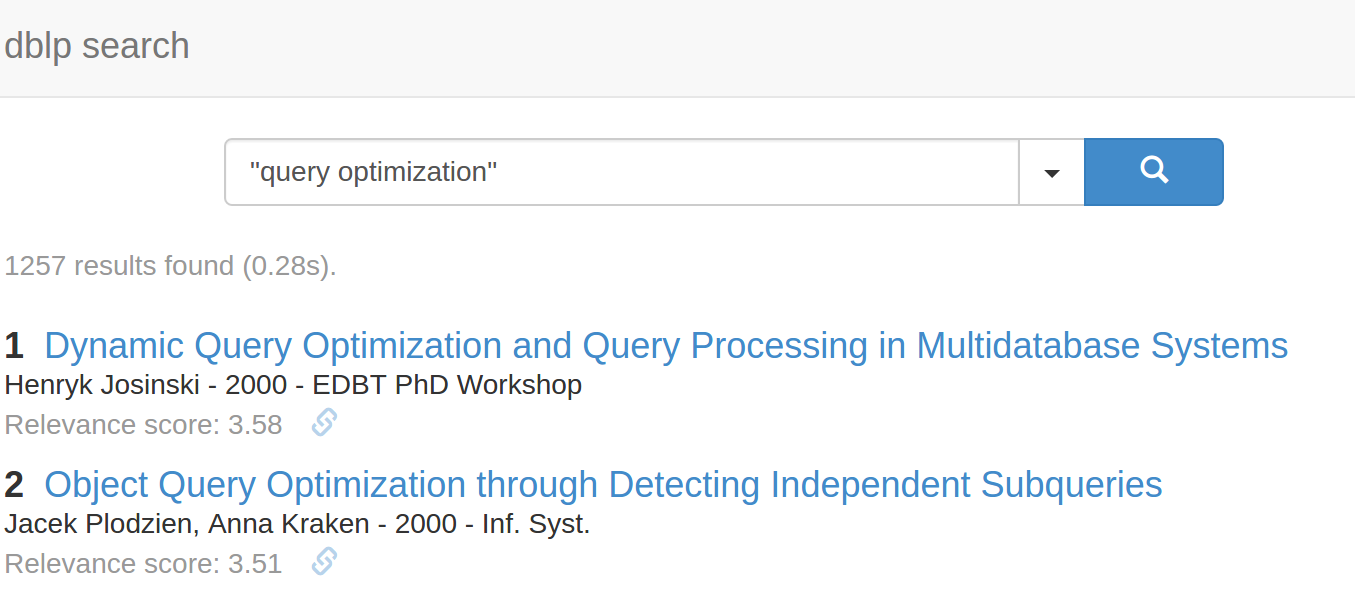
\includegraphics[width=0.48\textwidth]{img/search}
\label{fig:search}
\end{figure}  

\section{Applications in IR}

\subsection{Popular research topics}

\subsection{Similar publication venues}

\section{Conclusions}

%
% The following two commands are all you need in the
% initial runs of your .tex file to
% produce the bibliography for the citations in your paper.
\bibliographystyle{abbrv}
\bibliography{report}  % sigproc.bib is the name of the Bibliography in this case
% You must have a proper ".bib" file
%  and remember to run:
% latex bibtex latex latex
% to resolve all references
%

\end{document}
